\documentclass{beamer}
\mode<presentation>
{
  \usetheme{ldv}
  \setbeamercovered{transparent}
}

% Uncomment this if you're giving a presentation in german...
\usepackage[ngerman]{babel}

% ...and rename this to "Folie"
\newcommand{\slidenomenclature}{Folie}


\usepackage[utf8]{inputenc}
\usepackage{amsmath,amssymb,amsfonts}
\usepackage{times}
\usepackage{graphicx}
\usepackage{fancyvrb}
\usepackage{array}
\usepackage{colortbl}
\usepackage{tabularx}

% Uncomment me when you need to insert code
\usepackage{color}
\usepackage{listings}
\usepackage{minted}
\usepackage{algpseudocode}
% End Code

\usepackage{datetime}
\usepackage{tikz}
\usepackage{xcolor}
\usepackage{enumitem}

\usetikzlibrary{calc}
\usetikzlibrary{shapes.geometric}
\usetikzlibrary{decorations.pathreplacing}

\lstset{basicstyle=\ttfamily}

% Uncomment me when you need video or sound
% \usepackage{multimedia}
% \usepackage{hyperref}
% End video

% Header
\newcommand{\zwischentitel}{Woche 12}
\newcommand{\leitthema}{Tobias Eppacher}
\newcommand{\presdatum}{\formatdate{14}{7}{2025}}
% End Header

% Titlepage
\title{Grundlagen: Algorithmen und Datenstrukturen}
\author{Tobias Eppacher}
\date{\presdatum}
\institute{School of Computation, Information and Technology}
\subtitle{Woche 12}
% End Titlepage


% Slides
\begin{document}


% 1. Slide: Titlepage
\begin{frame}
	\titlepage
\end{frame}

% 2. Slide: TOC
\begin{frame}
	\frametitle{Inhalt}
	\tableofcontents[subsectionstyle=hide]
\end{frame}

\section{Aufgaben}

\begin{frame}
	\frametitle{Aufgabe 13.1 - Dijkstra}
	\scriptsize
	Führen Sie den Algorithmus von Dijkstra auf dem folgenden Graphen durch, um jeweils einen
	kürzesten Weg von $s$ zu jedem anderen Knoten zu finden. Protokollieren Sie nachvollziehbar Ihre Vorgehensweise, und markieren Sie zum Schluss alle Kanten, die zum gefundenen
	Kürzeste-Wege-Baum gehören.
	\begin{center}
		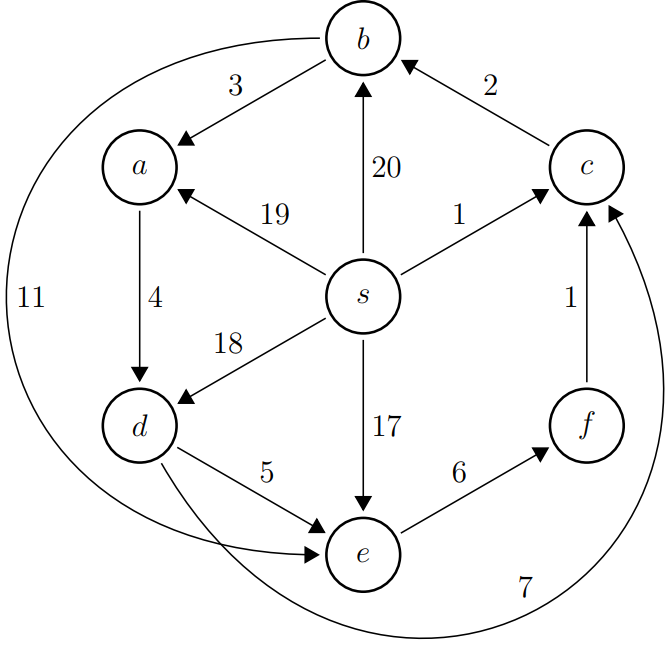
\includegraphics[width=0.55\textwidth]{images/dijkstra.png}
	\end{center}
\end{frame}

\begin{frame}
	\frametitle{Aufgabe 13.1 - Dijkstra}
	\begin{columns}
		\begin{column}{0.75\textwidth}
			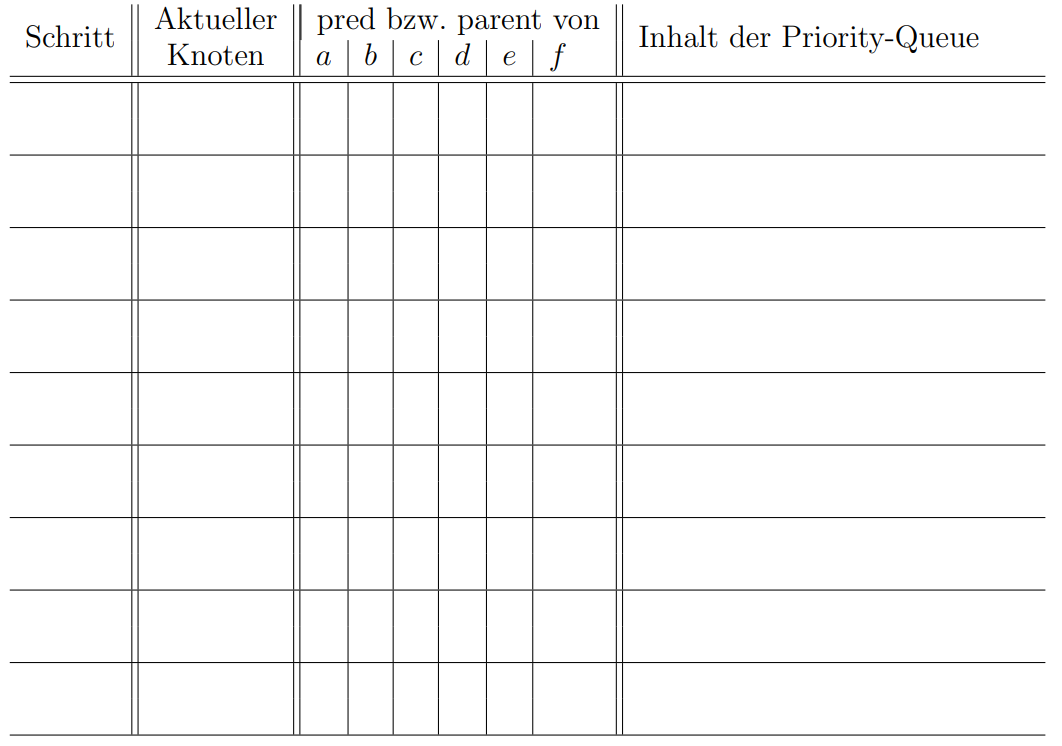
\includegraphics[width=\textwidth]{images/dijkstra_table.png}
		\end{column}
		\begin{column}{0.33\textwidth}
			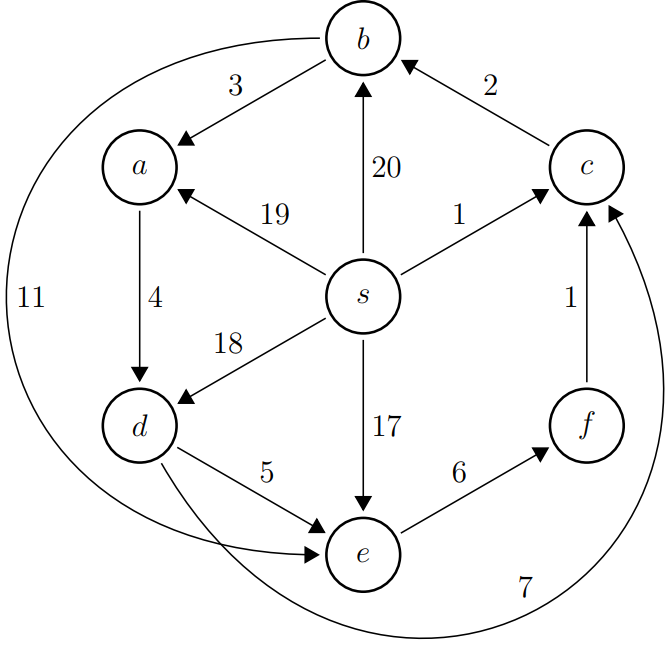
\includegraphics[width=\textwidth]{images/dijkstra.png}
		\end{column}
	\end{columns}
\end{frame}

\begin{frame}
	\frametitle{Aufgabe 13.2 - Bellman Ford}
	Führen Sie den Bellman-Ford-Algorithmus auf folgendem Graphen aus:
	\begin{center}
		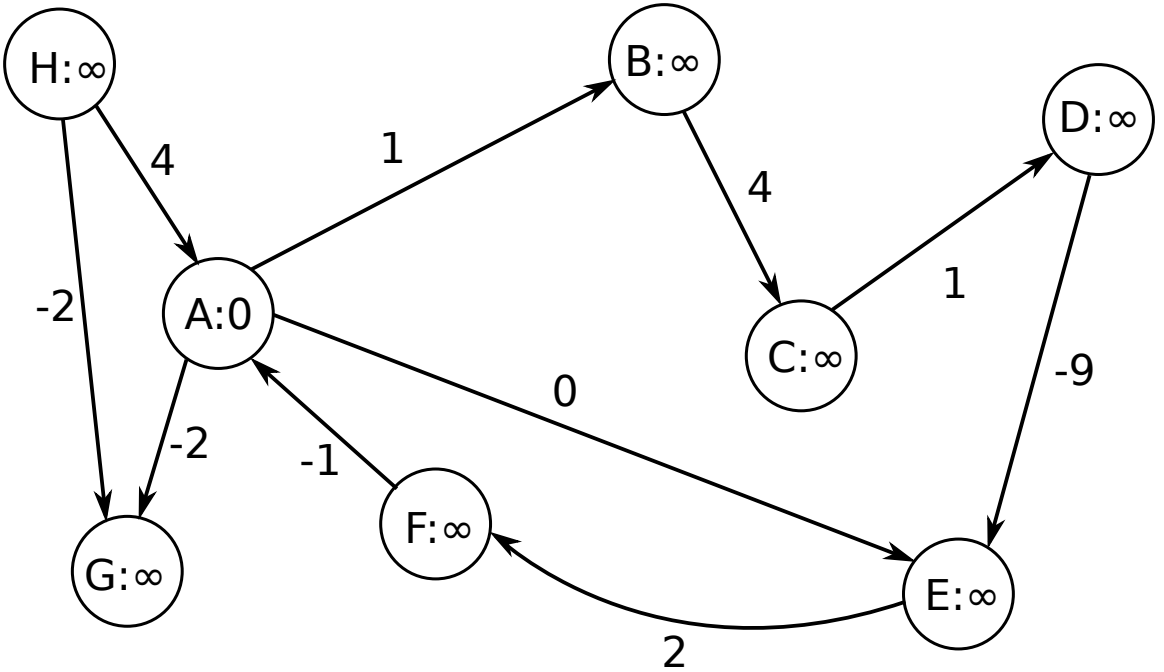
\includegraphics[width=0.8\textwidth]{images/bellman_ford.png}
	\end{center}
\end{frame}

\begin{frame}
	\frametitle{Aufgabe 13.2 - Bellman Ford}
	Schritt 1:
	\begin{center}
		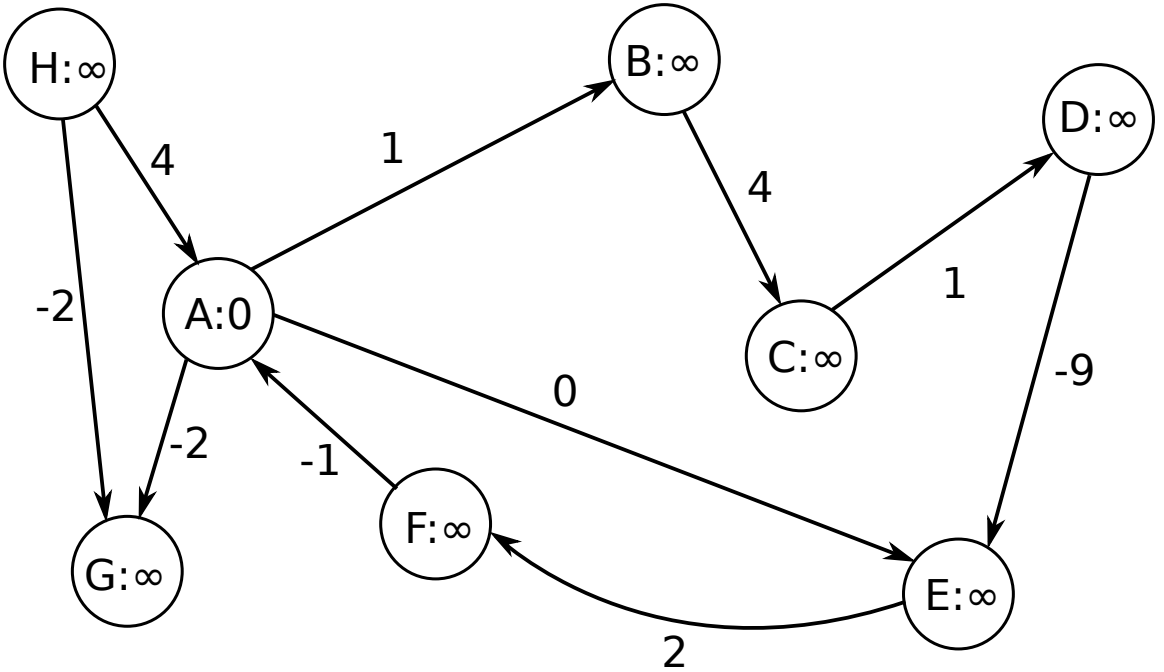
\includegraphics[width=0.8\textwidth]{images/bellman_ford.png}
	\end{center}
\end{frame}

\begin{frame}
	\frametitle{Aufgabe 13.2 - Bellman Ford}
	Schritt 2:
	\begin{center}
		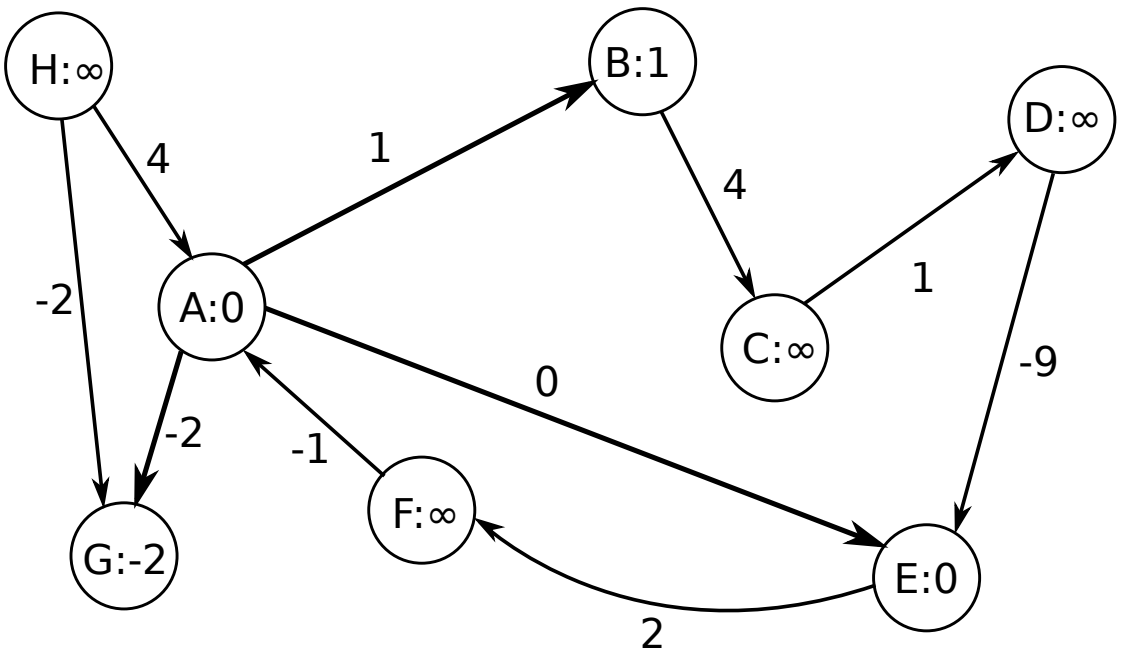
\includegraphics[width=0.8\textwidth]{images/bellman_ford1.png}
	\end{center}
\end{frame}

\begin{frame}
	\frametitle{Aufgabe 13.2 - Bellman Ford}
	Schritt 3:
	\begin{center}
		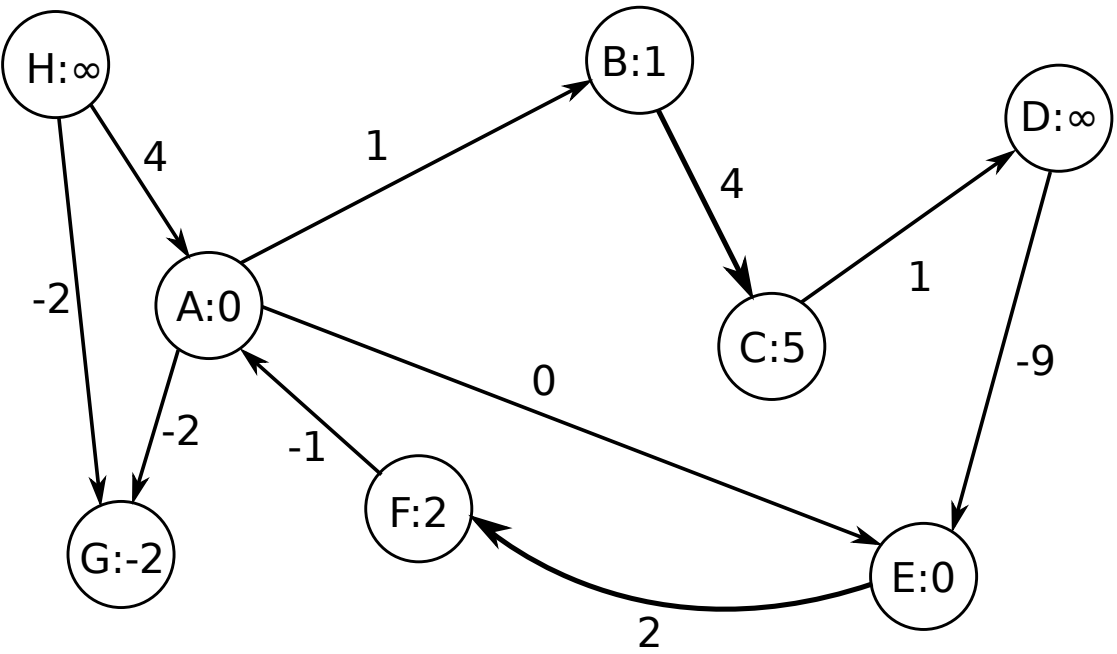
\includegraphics[width=0.8\textwidth]{images/bellman_ford2.png}
	\end{center}
\end{frame}

\begin{frame}
	\frametitle{Aufgabe 13.2 - Bellman Ford}
	Schritt 4:
	\begin{center}
		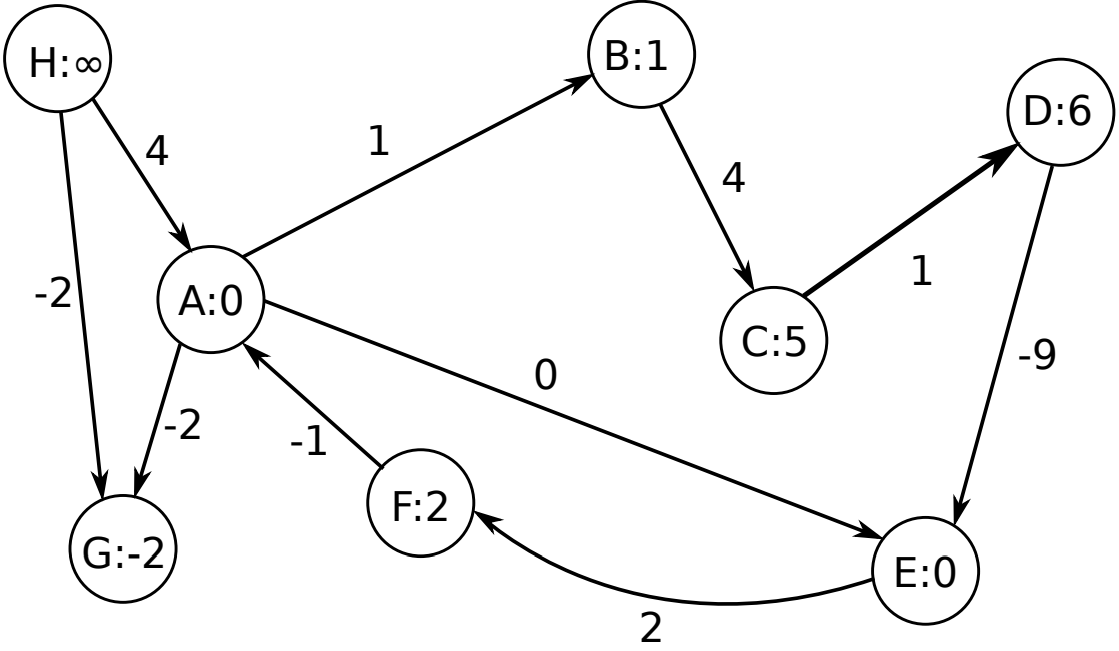
\includegraphics[width=0.8\textwidth]{images/bellman_ford3.png}
	\end{center}
\end{frame}

\begin{frame}
	\frametitle{Aufgabe 13.2 - Bellman Ford}
	Schritt 5:
	\begin{center}
		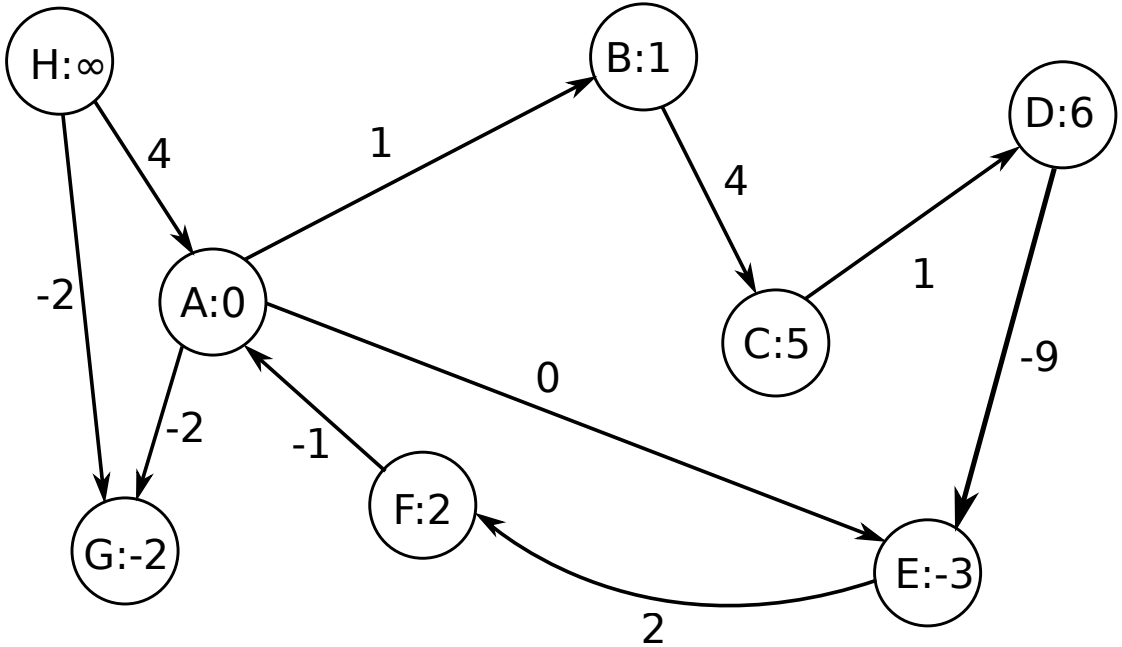
\includegraphics[width=0.8\textwidth]{images/bellman_ford4.png}
	\end{center}
\end{frame}

\begin{frame}
	\frametitle{Aufgabe 13.2 - Bellman Ford}
	Schritt 6:
	\begin{center}
		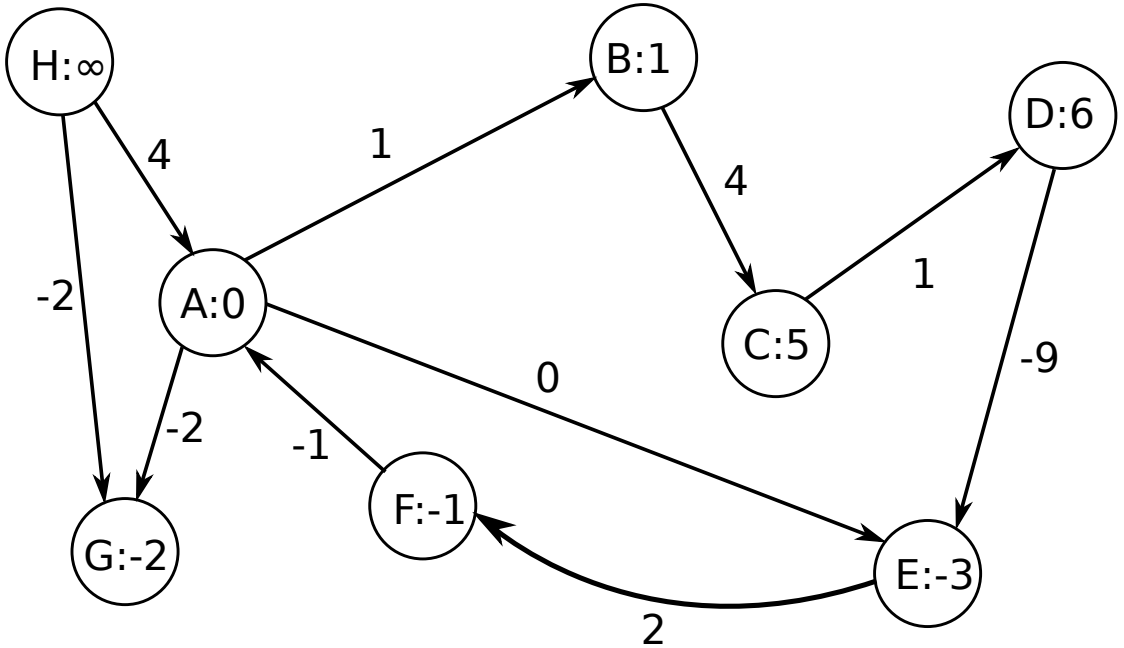
\includegraphics[width=0.8\textwidth]{images/bellman_ford5.png}
	\end{center}
\end{frame}

\begin{frame}
	\frametitle{Aufgabe 13.2 - Bellman Ford}
	Schritt 7:
	\begin{center}
		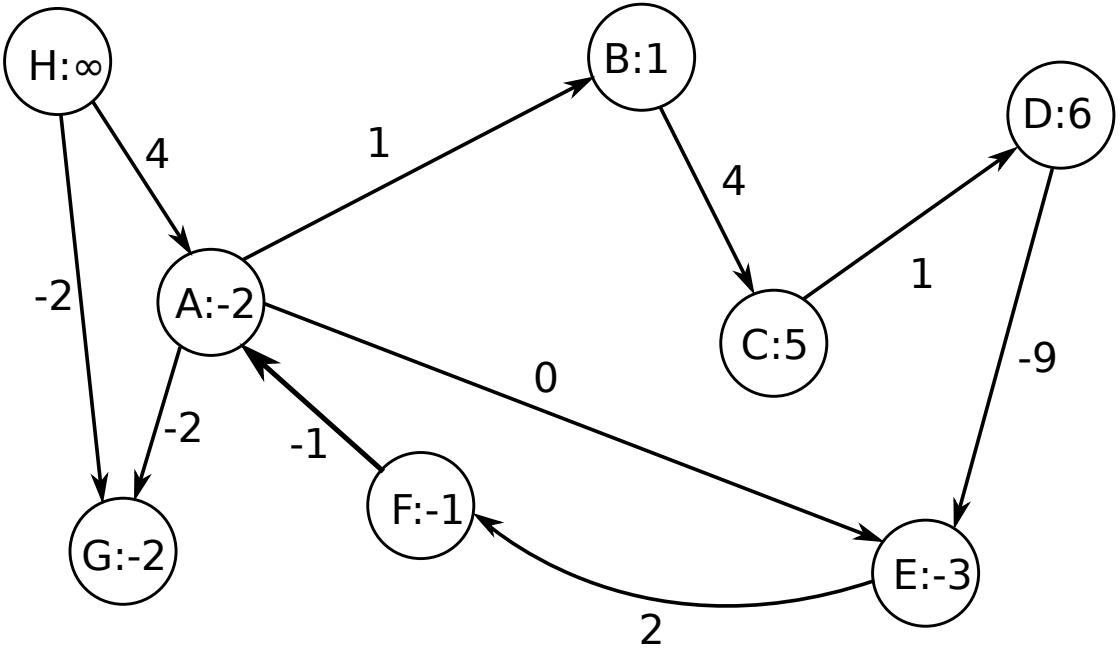
\includegraphics[width=0.8\textwidth]{images/bellman_ford6.png}
	\end{center}
\end{frame}

\begin{frame}
	\frametitle{Aufgabe 13.2 - Bellman Ford}
	Schritt 8 ($n$-te Iteration, infiziere Knoten):
	\begin{center}
		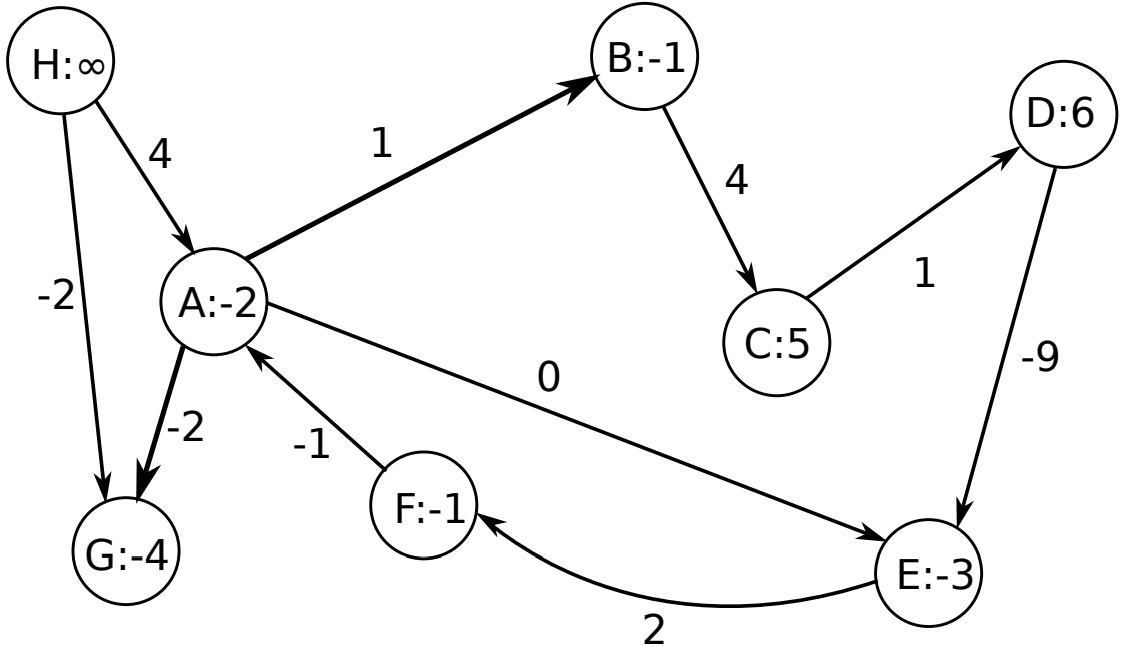
\includegraphics[width=0.8\textwidth]{images/bellman_ford7.png}
	\end{center}
\end{frame}

\begin{frame}
	\frametitle{Aufgabe 13.2 - Bellman Ford}
	Ausbreitung:
	\begin{center}
		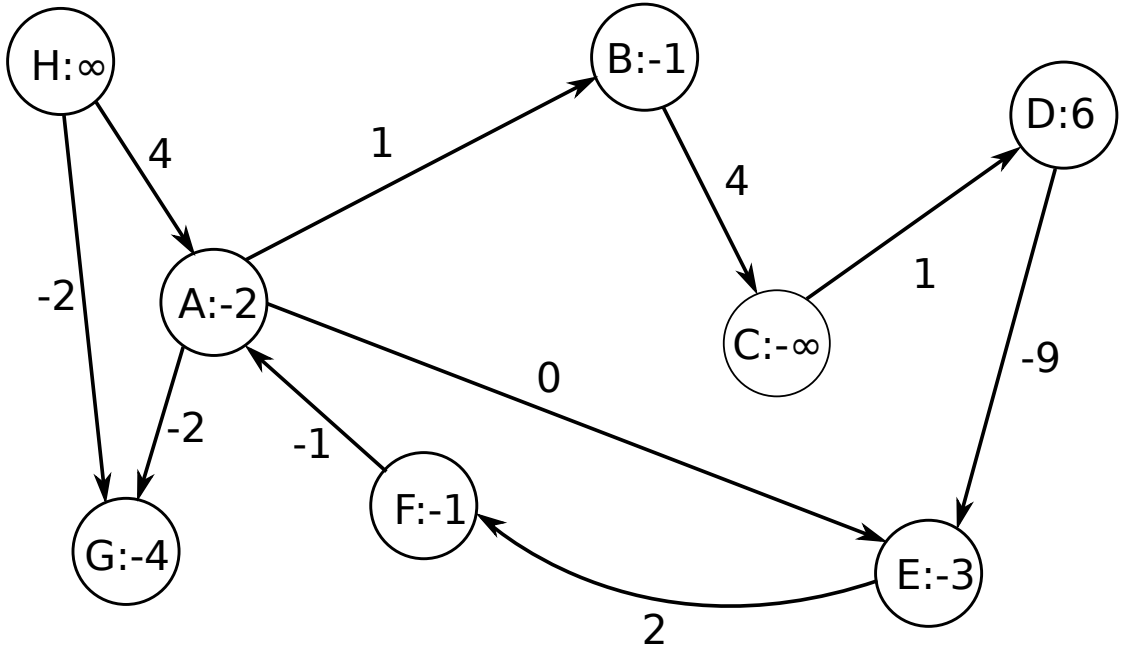
\includegraphics[width=0.8\textwidth]{images/bellman_ford_i1.png}
	\end{center}
\end{frame}

\begin{frame}
	\frametitle{Aufgabe 13.2 - Bellman Ford}
	Ausbreitung:
	\begin{center}
		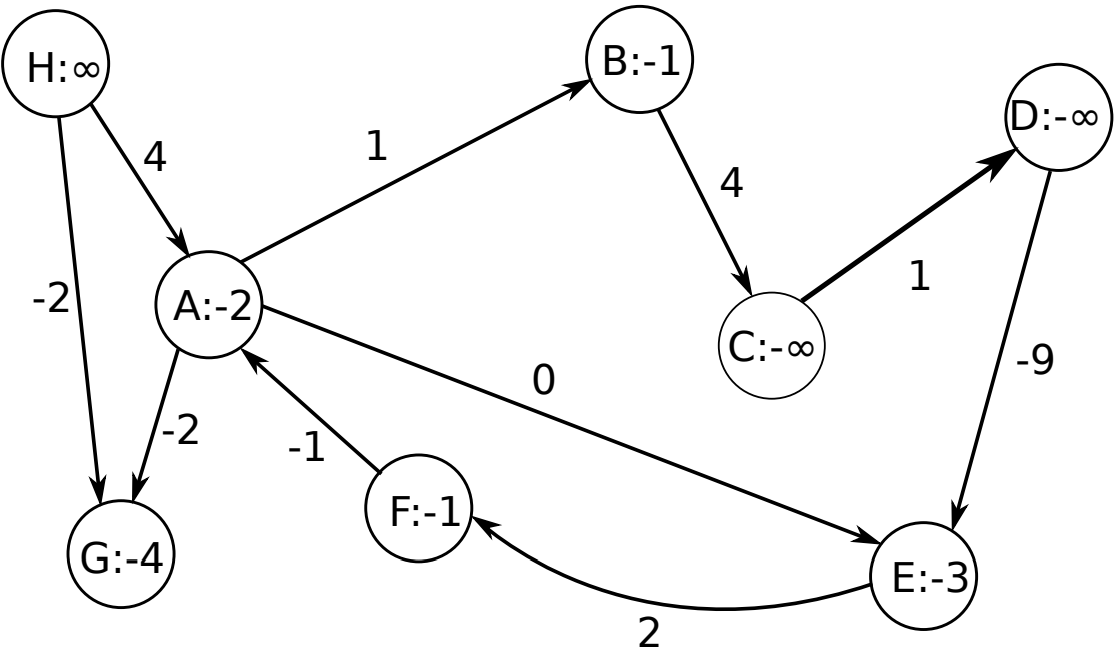
\includegraphics[width=0.8\textwidth]{images/bellman_ford_i2.png}
	\end{center}
\end{frame}

\begin{frame}
	\frametitle{Aufgabe 13.2 - Bellman Ford}
	Ausbreitung:
	\begin{center}
		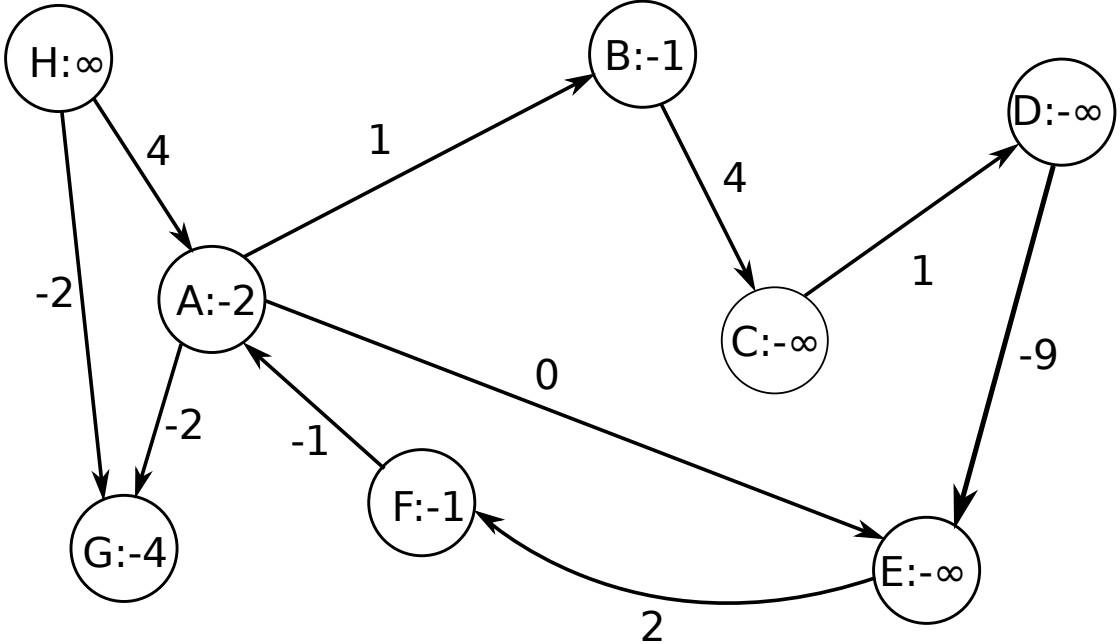
\includegraphics[width=0.8\textwidth]{images/bellman_ford_i3.png}
	\end{center}
\end{frame}

\begin{frame}
	\frametitle{Aufgabe 13.2 - Bellman Ford}
	Ausbreitung:
	\begin{center}
		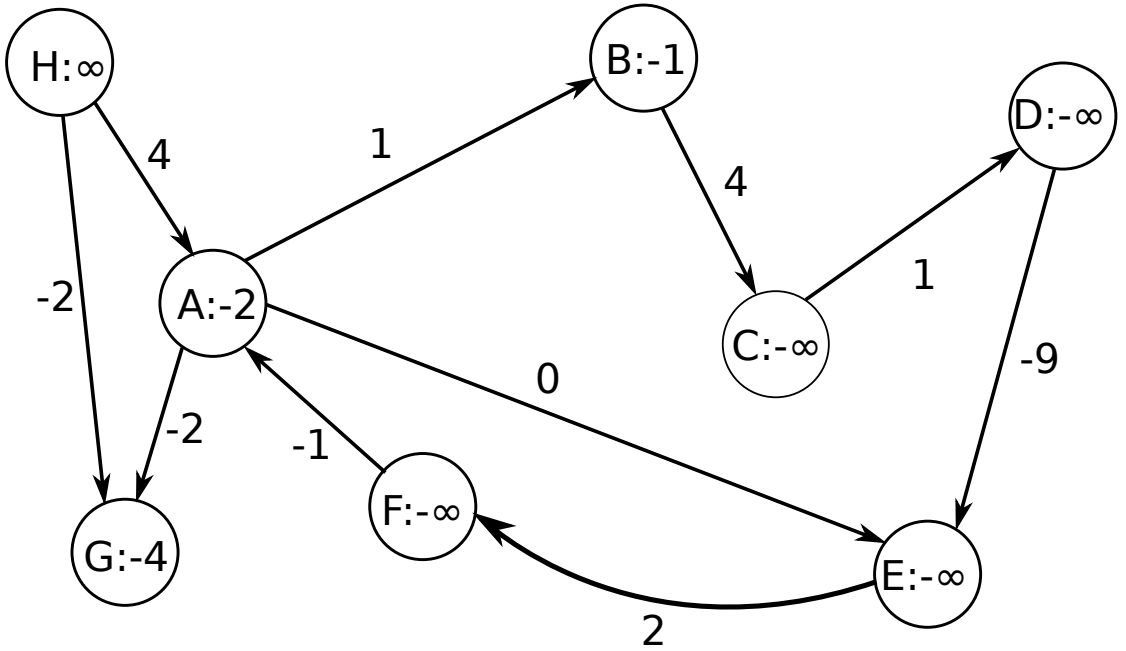
\includegraphics[width=0.8\textwidth]{images/bellman_ford_i4.png}
	\end{center}
\end{frame}

\begin{frame}
	\frametitle{Aufgabe 13.2 - Bellman Ford}
	Ausbreitung:
	\begin{center}
		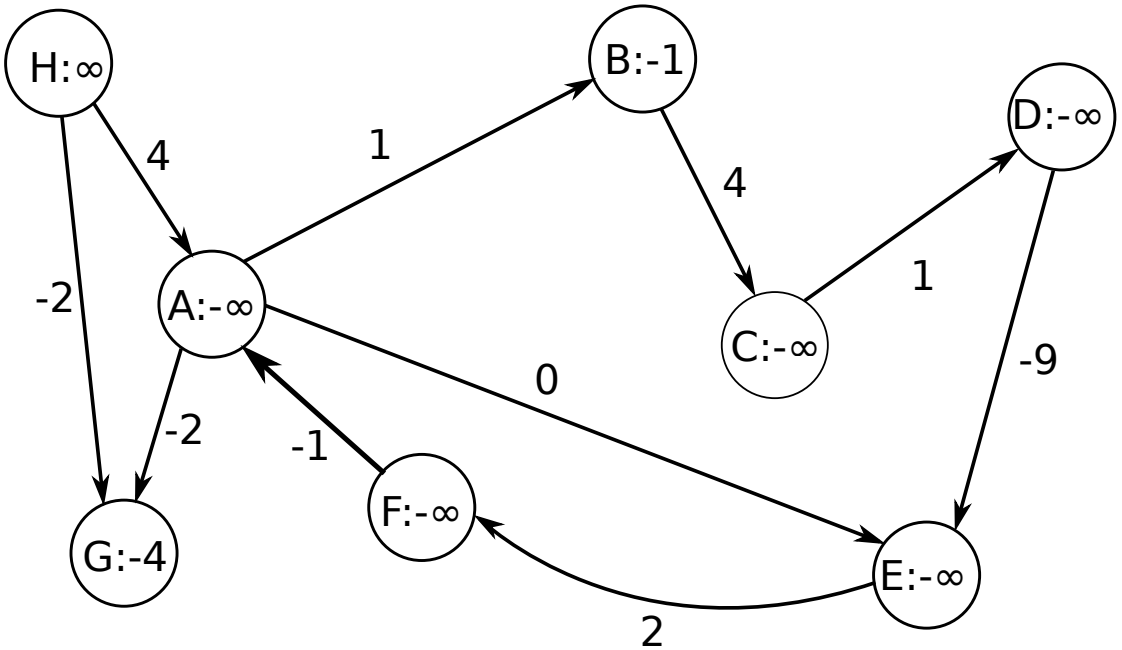
\includegraphics[width=0.8\textwidth]{images/bellman_ford_i5.png}
	\end{center}
\end{frame}

\begin{frame}
	\frametitle{Aufgabe 13.2 - Bellman Ford}
	Ausbreitung:
	\begin{center}
		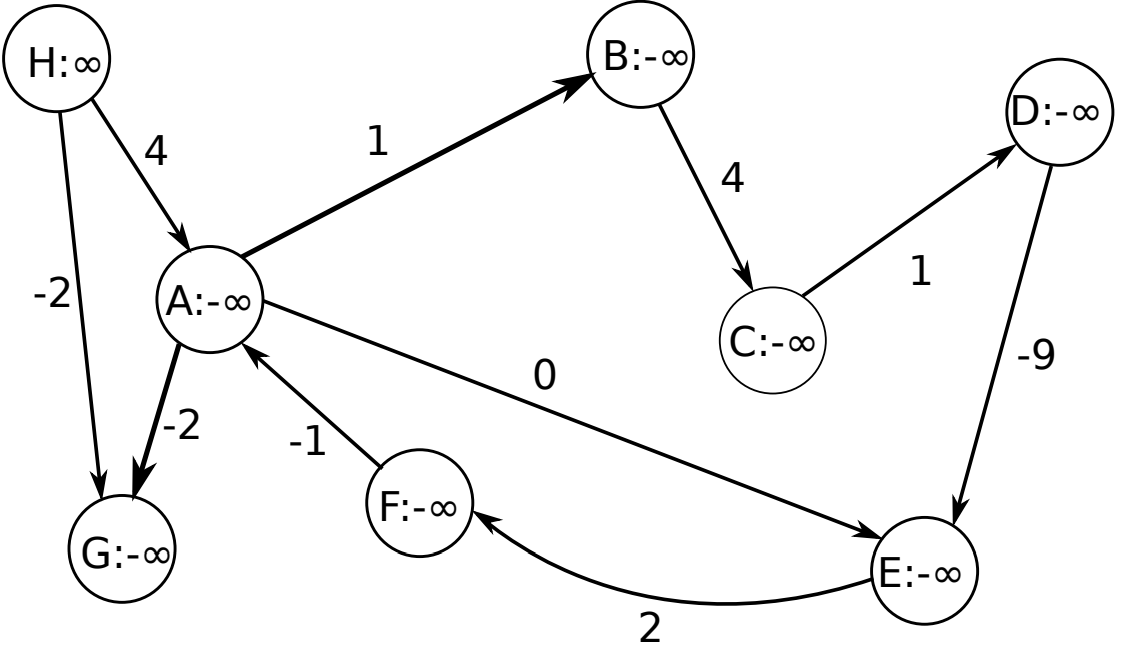
\includegraphics[width=0.8\textwidth]{images/bellman_ford_i6.png}
	\end{center}
\end{frame}

\section{E-Aufgaben}
\begin{frame}
	\frametitle{E-Aufgaben}
	\begin{itemize}
		\item Aufgabe 13.4 - Dijana und Stratos
	\end{itemize}
\end{frame}

\section{Hausaufgaben}
\begin{frame}
	\frametitle{Hausaufgaben}
	\begin{itemize}
		\item Hausaufgabe 11 - Double Hashing \\
		      (Deadline: 23.07.2025)
		\item Hausaufgabe 12 - Graphen \\
		      (Deadline: 30.07.2025)
	\end{itemize}
\end{frame}

\begin{frame}{\null}
	\huge
	\begin{center}
		Danke für's Dabeisein!
	\end{center}
\end{frame}

\begin{frame}{\null}
	\huge
	\begin{center}
		Viel Erfolg bei den Klausuren!
	\end{center}
\end{frame}

% End Slides

\end{document}
